%This is the first/leading file on the whole ``Data_Analysis Chapter
%Created by kp on Sep 8, 2013

\hspace{0.5cm}

\section{Raw Data Processing - Calibration and Reconstruction}   %Calibration and Reconstruction?
\begin{comment}
The raw data recorded by the CLAS DAQ system consist of ADC and TDC values registered by different components of the detector (in response to the passing of various particles through them) and also some beam related information such as Faraday Cup readings and beam helicity information. These data are collected and saved (by the DAQ system) in the fortran-77 based BOS format \cite{bos} which implements a dynamic memory management. %citation needed here (De Vita tesi, 51/65)
In the BOS file, the data is organized into banks, with each bank carrying data belonging to a particular detector or some part of it. Each bank consists of two parts - header and body. The body contains the actual collected data (such as the ADC and TDC values from detector components such as PMTs, in the case of raw data, or information such as energy and time in case of the reconstructed data), while %but 
the header contains some relational information - such as the bank identifier, the number of rows and columns of data in the bank and the location of the next bank. In the case of reconstructed data, in addition to the banks carrying detector specific reconstructed information such as the energy and time of the signals, more banks are added to the data file for storing high level information such as the number of particles detected in a given event, the four-momenta of each of the particles etc. 
\end{comment}

The raw data recorded by the CLAS DAQ system, which consists of ADC and TDC values registered by various detector components as well as the beam related information such as beam helicity and Faraday Cup readings, are organized into banks (with each bank carrying data belonging to a particular detector component or some part of it) and saved in special format (BOS) files. These raw data are next processed with a standard CLAS software package called RECSIS, which analyzes and combines the matching bits and pieces of the raw information to reconstruct particles and events that produced them. Such reconstruction produces output data that consist of event and particle IDs, particle positions and energies and momenta (in the lab frame CLAS coordinate system), and also some static particle properties such as charge and mass. The reconstruction program uses geometric parameters and calibration constants (from the %available 
CLAS Calibration Database) for the detector %(determined separately) 
in order to properly process and transform the raw data into the reconstructed tracks.


The first part of the data processing is the detector calibration. In this phase, a small sample (about 10\%) of raw data (uniformly selected over the entire run period to ensure time stability verification) is chosen and the energy and time calibration constants are adjusted to give the correct behavior while constantly monitoring related variables. This is done separately for each run period to consider the different running conditions, the possibility of unwanted changes in hardware that may have occurred, as well as drift of detector response over time. This process of adjusting the calibration constants and reconstructing the data is repeated until a desired level of accuracy is reached. Once that level is reached, the calibration constants are ``frozen'' and the final reconstruction is done. The resulting output is saved in especial formats\footnote{Two especial data formats - BOS and ntuple (h10) - were used}. 

These saved data provided the starting point for our higher level data analysis as described in this dissertation. The details of the calibration and reconstruction process can be found in \cite{rdVita_th}.

The iterative work of data reconstruction and detector calibration, which was a very computing intensive and time consuming, was done by R. De Vita - one of the EG4 collaborators from  INFN, Genova, with good expertise on CLAS data reconstruction - soon after the data collection was completed (from 2006-2007). The data from this ``Pass1'' reconstruction was first analyzed as part of the Ph. D. dissertations by three graduate students, but during these analyses, a few anomalies\footnote{The anomalies observed in the pass1 analysis were the discretized reconstruction of vertex and wrong reconstruction of track positions in DC1.} in reconstruction were observed which were later tracked down to a %https://clasweb.jlab.org/rungroups/eg4/wiki/index.php/User:Lamiaa#EG4_Software_Update_.26_Solution
mixing up of codes from two EG4 sub-packages for the reconstruction software. After the mix-up was sorted out, a new pass (Pass2) of reconstruction was performed by L. El Fassi (still using the same calibration constants as used by the Pass1 reconstruction). The data from this latest pass of reconstruction was used for the analysis reported in this note 


\section{Helicity States}

%\textcolor{red}{More to be done.}
\begin{figure}[H]%[h] %ht, htpb (p - float, b = bottom, h=? t = top)
  \centering
  \leavevmode 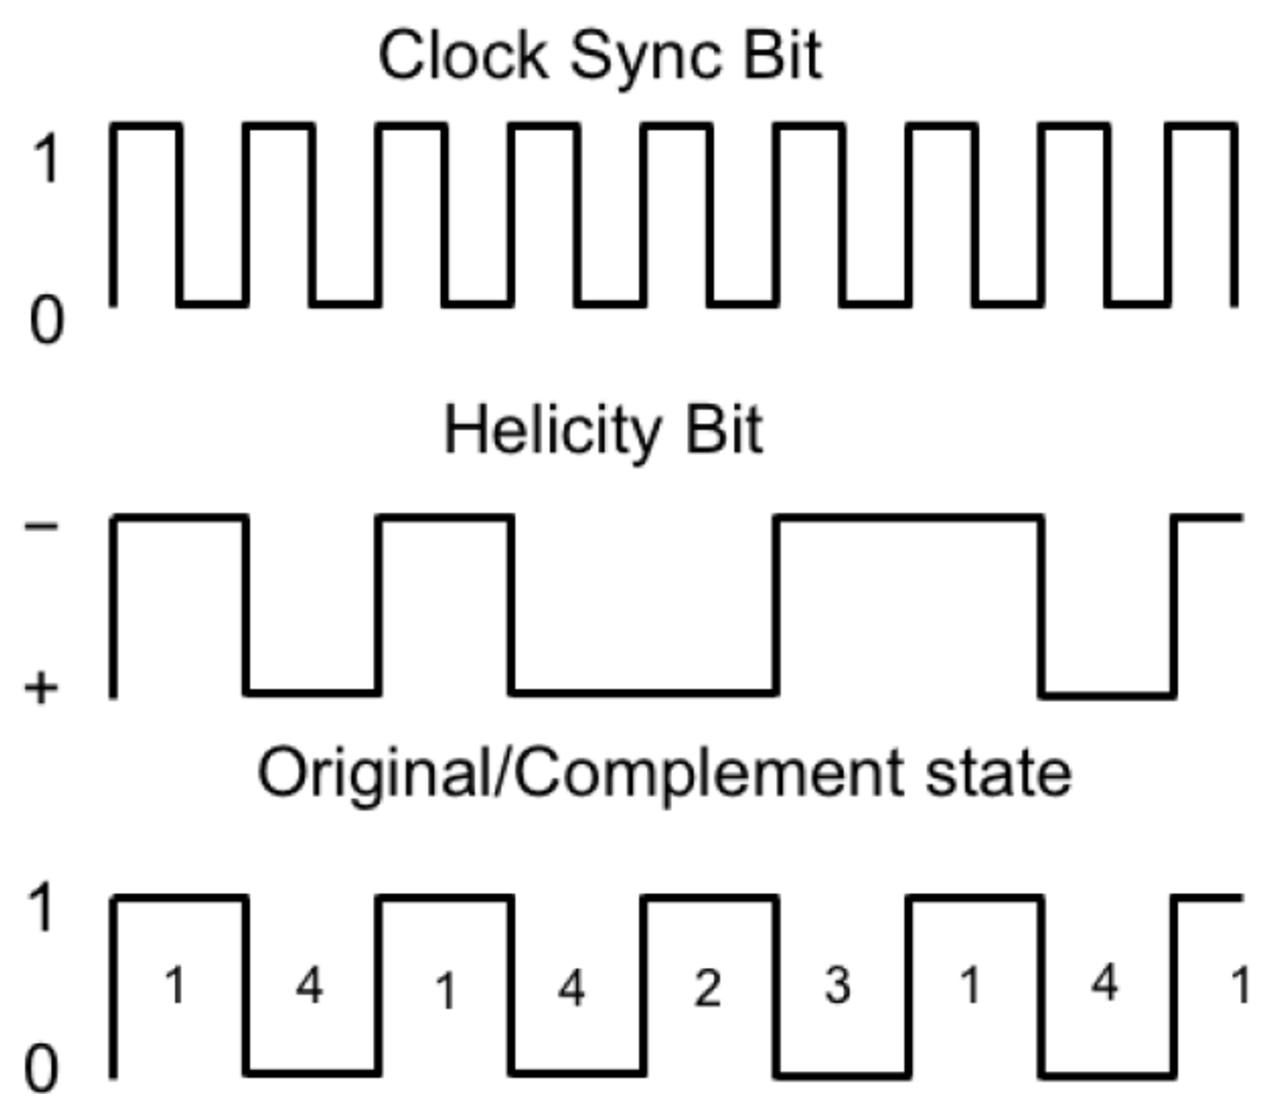
\includegraphics[width=0.4\textwidth]{figuresEG4/FigSim/helicityPairingNevzatCut} 
  \caption[Helicity Pairing]{Different data signals sent from the injector that monitor the helicity states of beam electrons. (Fig. courtesy of N. Guler \cite{nGuler_th} ).}
  \label{figHeli}
\end{figure}
%Prok pg 138, https://clasweb.jlab.org/rungroups/eg4/wiki/index.php/User:Devita; Sulkosky pg 70

As we saw from Eq. \ref{eqXSdiff}, the physics %quantity 
extraction depends on %the
measurements of the number of events in %counts for 
the two (+/-) electron helicity states. The CEBAF accelerator provides the polarized electrons in closely and % but 
equally spaced bunches. These bunches are further grouped into ``buckets'' according to their helicity states, which are %is 
alternated pseudo-randomly at the injector with a frequency of 30 Hz. The information on the helicity state of each of the buckets and the total integrated charge contained in it is injected into the DAQ data stream immediately after the helicity flip. Using a combination of different types of sequence control signals sent from the injector (see Fig. \ref{figHeli}), it is possible to determine which helicity state a particular event belonged to, which then can be used to label the helicity state of the event in the data stream, %its 'HEAD' bank, 
together with the total beam charge of the state.


\begin{comment}
This is called the original state. The original state is always followed by a complement state. The information about the helicity state and the total integrated charge for that helicity state are stored in the data stream after each helicity flip (sometimes the information was injected after 2 helicity flips depending on the DAQ throughput). A sync pulse, with twice the frequency of the helicity pulse, is also delivered to the experimental hall and stored in the data stream. The sync pulse is used to identify the helicity flips and detect missing helicity bits. The original helicity state is always labeled with 1 or 2, while the complement state is labeled with 3 or 4. The original helicity pulse labeled with 1 should always be followed by a complement helicity pulse labeled with 4. Similarly, 2 should always be followed by 3. The flip should always coincide with the rising edge of every other sync pulse. Fig. \ref{figHeli} shows the flow of helicity states together with corresponding helicity bits labeled with + or − . Knowing the order of helicity labels, one can identify if any helicity state was missed due to dead time problems in the DAQ system. A broken sequence leads to unpaired helicity states, which would introduce a false asymmetry. It was determined that the helicity label stored in each physics event sometimes failed to latch leading to a broken sequence. Fortunately, the Faraday Cup scaler had its own helicity label latch which did not fail. The information from the FC scalers was used to recover the correct sequence.


An algorithm, as a part of the “HelP.cc” [92] program, was designed to track down the helicity states and determine the problematic helicity buckets. The algorithm was incorporated as a part of the DST library and the necessary flags to identify correct helicity sequencing were written into the DST files. The code extracts the helicity in terms of 1 or 0 or a number less than 0, which indicates that the helicity state is suspect. 5 The negative values are encoded according to the list in Table 6. While processing the DST files for analysis, a program called PATCH was used to produces tables for each DST data file to monitor the helicity sequence and throw
away bad helicity buckets. The tables produced by PATCH include minimum and maximum event numbers for each helicity bucket together with the labels of original or complement states and the corresponding helicity bits determined by the HelP algorithm. The table also includes the minimum and maximum event numbers from scaler BANKS in the DST and finally a flag for the helicity bucket indicating whether it is good (flag = 1) or bad (flag = 10,-1000). The PATCH program labels any helicity state smaller than 1 or larger than 4 with -10. These states will be disregarded from further analysis. The program also examines the order of the helicity states and determines the buckets that are out of sequence. It also compares minimum and maximum event numbers from the trigger banks with the output of the scaler banks and labels unmatched helicity buckets. The label for these two latter cases is - 1000. In addition, PATCH takes care of suspicious helicity states at the end of some DST files that occur during file closing. Whenever a bad helicity bucket is found, the original and the complement states are always thrown away together until the correct sequence is recovered. This ensures that the removal of problematic buckets will not bias any particular helicity state. During the analysis process, the PATCH program is executed first and its output table is used by the DST reader to determine problematic helicity buckets. A segment from its output is shown in Table 7.
\end{comment}
